% In order to demonstrate the scalability and performance of HTBAC we will
% focus on the ESMACS protocol alone applied to a representative kinase
% system.

% ---------------------------------------------------------------------------
\subsection{Protocols for Binding Affinity Calculations}

We have demonstrated the lack of reproducibility of single trajectory
approaches in both HIV-1 protease and MHC systems, with calculations for the
same protein-ligand combination, with identical initial structure and force
field, shown to produce binding affinities varying by up to 12 kcal mol
$^{-1}$ for small ligands (flexible ligands can vary even
more)~\cite{Wan2015, Sadiq2010, Wright2014}. Indeed, our work has revealed
how completely unreliable single simulation based approaches are.

Our work using ensemble simulations have also reliably produced results in
agreement with previously published experimental findings~\cite{Sadiq2010,
Wan2011, Wright2014, Bhati2017, Wan2017brd4, Wan2017trk}, and correctly
predicted the results of experimental studies performed by colleagues in
collaboration~\cite{Bunney2015}. While the accuracy of force fields could be a
source of error, we know from our work to date that the very large
fluctuations in trajectory-based calculations account for the lion’s share of
the variance (hence also uncertainty) of the results.

% Almost all MMPBSA studies in the literature use the so-called 1-trajectory
% method, in which the energies of protein-inhibitor complexes, receptor
% proteins and ligands are extracted from the MD trajectories of the
% complexes alone. ESMACS protocols can additionally use separate ligand and
% receptor trajectories to account for adaptation energies.


% ---------------------------------------------------------------------------
% \subsubsection*{ESMACS}

We designed two free energy calculation protocols with the demands of clinical
decision support and drug design applications in mind: ESMACS (enhanced
sampling of molecular dynamics with approximation of continuum
solvent)~\cite{Wan2017brd4} and TIES (thermodynamic integration with enhanced
sampling)~\cite{Bhati2017}. The former protocol is based on variants of the
molecular mechanics Poisson-Boltzmann surface area (MMPBSA) end-point method,
the latter on the `alchemical' thermodynamic integration (TI) approach. In
both cases, ensembles of MD simulations are employed to perform averaging and
to obtain tight control of error bounds in our estimates. In addition, the
ability to run replica simulations concurrently means that, as long as
sufficient compute resources are available, turn around times can be
significantly reduced compared to the generation of single long trajectories.
The common philosophy behind the two protocols entails similar middleware
requirements: In this work we focus on the ESMACS protocol but all results are
applicable also to TIES.

Each replica within the ESMACS protocol consists of a series of simulation
steps followed by post production analysis. Generally, an ESMACS replica will
contain between 3 and 12 equilibration simulation steps followed by a
production MD run, all of which are conducted in the NAMD
package~\cite{Phillips2005}. The first step is system minimization, the
following steps involve the gradual release of positional constraints upon
the structure and the heating to a physiologically realistic temperature.
Upon completion of the MD simulation, free energy computation (via MMPBSA and
potentially normal mode analysis) is performed using
AmberTools~\cite{Case2005, MillerIII2012}.

The ESMACS protocol is highly customizable. Both the number of simulation replicas in the ensemble and the lengths of their runs can be varied to
obtain optimal performance for any given system. Using replicas that only
vary in the initial velocities assigned to the atoms of the system we have
defined a standard protocol which prescribes a 25 replica ensemble, each run
consisting of 2 ns of equilibration and 4 ns of production simulation. Our
protocol has produced bootstrap errors of below 1.5 kcal mol$^{-1}$ (despite
replica values varying by more than 10 kcal mol$^{-1}$) for a varied range of
systems including small molecules bound to kinases and more flexible peptide
ligands binding to MHC proteins \cite{Wan2015, Wright2014, Wan2017brd4}.
In these systems, the error we obtained more than halves between ensembles of
5 and 25 replicas but increases in ensemble size have generally produced only
small improvements. More generally though, there may be cases where it is
important to increase the sampling of phase space either through expanding
the ensemble or by considering multiple initial configurations.

The ESMACS protocol can also be extended to account for adaptation energies
involved in altering the conformation of the protein or ligand during
binding. Almost all MMPBSA studies in the literature use the so-called
1-trajectory method, in which the energies of protein-inhibitor complexes,
receptor proteins and ligands are extracted from the MD trajectories of the
complexes alone. The ESMACS protocol can additionally use separate ligand and
receptor trajectories to account for adaptation energies, providing further
motivation to deploy the protocol via flexible and scalable middleware.

% ---------------------------------------------------------------------------
\subsection{Benchmark kinase system}

\begin{figure}
  \centering
  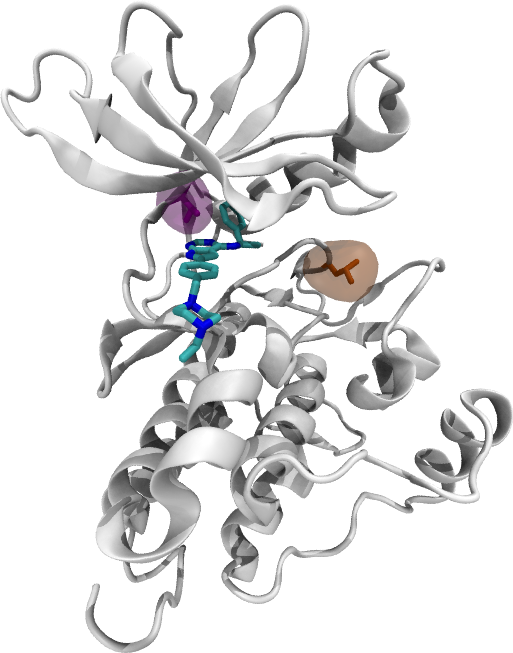
\includegraphics[width=0.60\columnwidth]{egfr.png}
  \caption{Cartoon representation of the EGFR kinase bound to the inhibitor
  AEE788 shown in chemical representation (based on PDB:2J6M). Two residues
  implicated in modulating drug efficacy are highlights; in pink T790 and in
  orange L858. Mutations to either of these residues significantly alter the
  sensitivity to TKIs.}\label{fig:egfr}
\end{figure}


A common target of kinase inhibitors is the epidermal growth factor receptor
(EGFR) which regulates important cellular processes including proliferation,
differentiation and apoptosis. EGFR is frequently over expressed in a range of
cancers, and is associated with disease progression and treatment. Clinical
studies have shown that EGFR mutations confer tumor sensitivity to tyrosine
kinase inhibitors in patients with non-small-cell lung cancer (examples shown
in Fig.~\ref{fig:egfr}) The tyrosine kinase domain of EGFR contains 288
residues, the full simulation system including solvent and the AEE788
inhibitor contains approximately 50 thousand atoms. The well established AMBER
ff99SBildn and GAFF force fields~\cite{Maier2015, Wang2004} were used to
parameterize the system for this work.
